\documentclass[border=2pt]{standalone}
\usepackage{tikz}
\usetikzlibrary{quotes,angles}
\usepackage{amsmath}

\begin{document}

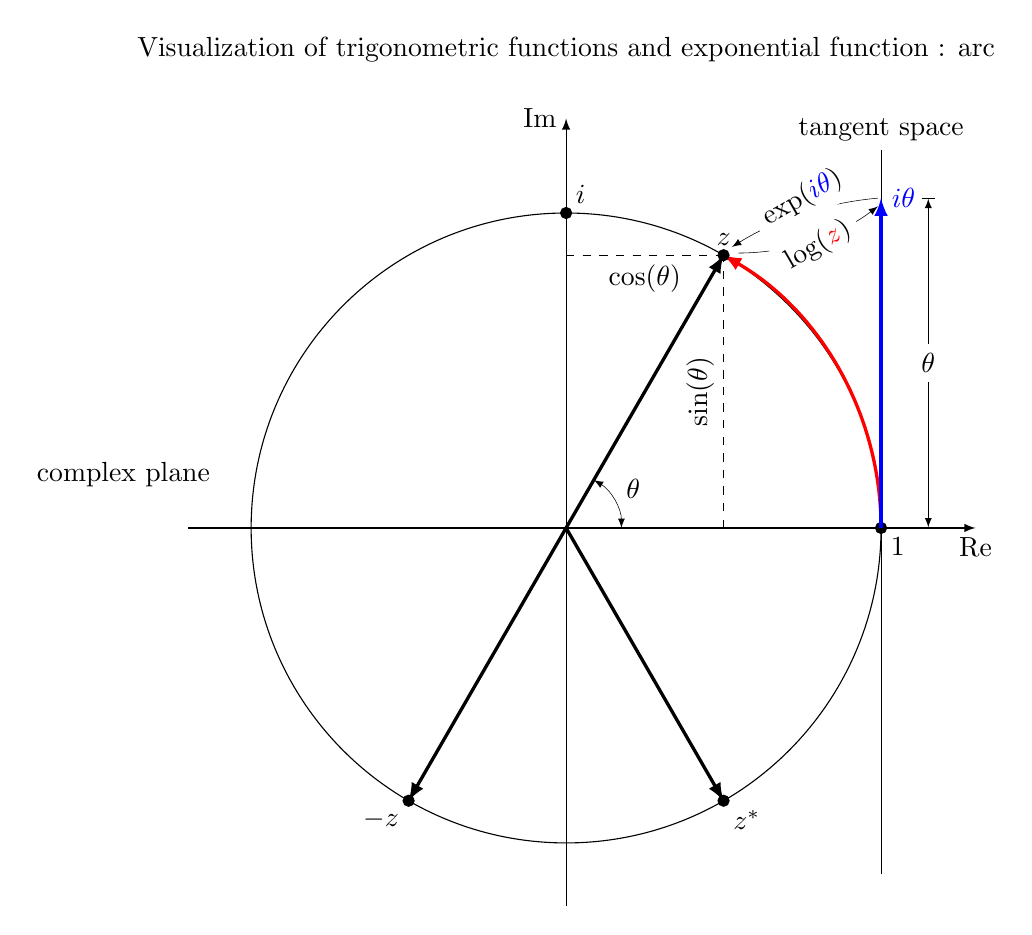
\begin{tikzpicture}[scale=4]

% Draw x and y axis lines
\draw [->,>=latex] (-1.2,0) -- (1.30,0) node [below] {$\mathrm{Re}$};
\draw [->,>=latex] (0,-1.2) -- (0,1.30) node [left ] {$\mathrm{Im}$};
\node[above left] at (-1.1, 0.1) {complex plane};
\filldraw[black] (1,0) circle (0.5pt) node[below right] {$1$} ;
\filldraw[black] (0,1) circle (0.5pt) node[above right] {$i$} ;
\node[above] at (0.0,1.45) {Visualization of trigonometric functions and exponential function : arc};

% Draw a circle at the origin of radius 1
\draw (0,0) circle (1);

\pgfmathsetmacro{\angle}{60}
	\pgfmathsetmacro{\length}{\angle / 180 * pi}

% Draw a red arc at the origin of radius 1
\draw [->,>=latex, very thick, red] (1,0) arc (0:\angle:1)
%	node[above] {$z$}
;

\draw
  (1,0) coordinate (a) 
  -- (0,0) coordinate (b) 
  -- ( {cos(\angle)}, {sin(\angle)} ) coordinate (c) 
  pic["$\theta$", draw=black, very thin, <->,>=latex, angle eccentricity=1.4, angle radius=20]
  {angle=a--b--c};


\draw [very thin, dashed] ( {cos(\angle)}, 0) -- node[above, rotate=90] {$\sin(\theta)$} ( {cos(\angle)}, {sin(\angle)}) ;
\draw [very thin, dashed] ( 0, {sin(\angle)}) -- node[below] {$\cos(\theta)$} ( {cos(\angle)}, {sin(\angle)}) ;

\draw [very thick,->,>=latex] (0,0) -- ( {cos(\angle)}, {sin(\angle)}) ;
\draw [very thick,->,>=latex] (0,0) -- ( {cos(\angle)},-{sin(\angle)}) ;
\filldraw[black] ( {cos(\angle)}, {sin(\angle)}) circle (0.5pt) node[above] {$z$} ;
\filldraw[black] ( {cos(\angle)},-{sin(\angle)}) circle (0.5pt) node[below right] {$z^*$} ;
\draw [very thick,->,>=latex] (0,0) -- (-{cos(\angle)},-{sin(\angle)}) ;
\filldraw[black] (-{cos(\angle)},-{sin(\angle)}) circle (0.5pt) node[below left] {$-z$} ;

% Draw a line at (1,0)
\draw [very thin] (1,-1.1) -- (1, 1.2) node[above] {tangent space};

\draw [->,>=latex] [very thick, blue] (1,0) -- (1, \length) node[right] {$i\theta$};
\draw [very thin, |<->|,>=latex] (1.15, 0) -- node[fill=white] {$\theta$} (1.15, \length);

\draw [very thin, ->,>=latex] (1.00 - 0.01, \length) arc (95:122:\length);
\draw ({cos(\angle)+0.25}, \length) node[fill=white, rotate=90-\angle] {$\exp(\color{blue}i\theta\color{black})$} ;

\draw [very thin, ->,>=latex] ( {cos(\angle)+0.45}, {sin(\angle)+0.41}, \length) arc (270:307:\length-0.31);
\draw ({cos(\angle)+0.30}, \length-0.15) node[fill=white, rotate=90-\angle] {$\log(\color{red}z\color{black})$} ;

\end{tikzpicture}

\end{document}

